\documentclass[10pt]{article}
\usepackage[verbose, a4paper, hmargin=2.5cm, vmargin=2.5cm]{geometry}

\usepackage{fontspec}
\usepackage{ctex}
\usepackage{paratype}


\usepackage{amsmath}
\usepackage{amsfonts}
\usepackage{amssymb}
\usepackage{esint}

\usepackage{graphicx}
\usepackage[export]{adjustbox}
\usepackage{mdframed}
\usepackage{booktabs,array,multirow}
\usepackage{adjustbox}
\usepackage{tabularx}
\usepackage{hyperref}
\hypersetup{colorlinks=true, linkcolor=blue, filecolor=magenta, urlcolor=cyan,}
\urlstyle{same}
\usepackage[most]{tcolorbox}
\definecolor{mygray}{RGB}{240,240,240}
\tcbset{
  colback=mygray,
  boxrule=0pt,
}
\graphicspath{ {./images/} }
\newcommand{\HRule}{\begin{center}\rule{0.9\linewidth}{0.2mm}\end{center}}
\newcommand{\customfootnote}[1]{
  \let\thefootnote\relax\footnotetext{#1}
}

\begin{document}
PAPER \(\cdot\) OPEN ACCESS

\section*{Machining Chatter Analysis for High Speed Milling Operations}

To cite this article: M. Sekar et al 2017 IOP Conf. Ser.: Mater. Sci. Eng. 247 012014

View the article online for updates and enhancements. UNITED THROUGH SCIENCE \& TECHNOLOGY IOP Conf. Series: Materials Science and Engineering 247 (2017) 012014 doi:10.1088/1757-899X/247/1/012014 Machining Chatter Analysis for High Speed Milling Operations M. Sekar* Department of Mechanical Engineering GMR Institute of Technology, Rajam, India mailtosekar@gmail.com I. Kantharaj Department of Mechanical Engineering Karunya University, Coimbatore, India kantharaj@karunya.edu

The Electrochemical Society Science + Technology+ 248th ECS Meeting Chicago, IL October 12-16, 2025 SUBMIT SUBMIT NOW

\begin{center}

\includegraphics[max width=1.0\textwidth]{images/01948e67-2b92-7dd1-b16f-a9746c8d80be_0_87_2083_1464_118_0.jpg}
\end{center}
\hspace*{3em} 

Savale Amit Siddhappa

Department of Mechanical Engineering Karunya University, Coimbatore, India amit.savale5@gmail.com

\section*{ABSTRACT}

Chatter in high speed milling is characterized by time delay differential equations (DDE). Since closed form solution exists only for simple cases, the governing non-linear DDEs of chatter problems are solved by various numerical methods. Custom codes to solve DDEs are tedious to build, implement and not error free and robust. On the other hand, software packages provide solution to DDEs, however they are not straight forward to implement. In this paper an easy way to solve DDE of chatter in milling is proposed and implemented with MATLAB. Time domain solution permits the study and model of non-linear effects of chatter vibration with ease. Time domain results are presented for various stable and unstable conditions of cut and compared with stability lobe diagrams.

Keywords- Delay Differential equations, Regenerative Chatter, R-K method.

\section*{I. INTRODUCTION}

The term High Speed Machining (HSM) commonly refers to end milling at high rotational speeds and high surface feeds [1]. High speed machining (HSM) is increasingly used to machine complex profiles with a goal of reducing lead times [2]. Machining Aero Engine parts and thin walled Jet Engine components in HSM is always prone to non-linear chatter vibrations as geometry changes abruptly and acceleration becomes out of machine tool limits. The ever increasing need of productivity and quality has made chatter an important area of research since 1960s. Machine tool chatter arises due to forced and self-excited vibrations. Tlusty [1] proved that the regenerative effect due to feedback effects of workpiece geometry from the previous tool pass is the major source of machine tool chatter. Regenerative chatter occurs when the cutting tool removes a surface with undulations created by an earlier tool pass. The associated change in chip thickness results in a varying dynamic cutting force resulting in a wavy surface accompanied with vibration which eventually leads to unstable machining process. Merrit [2] modeled this process in the form of a block diagram with feedback loop and solved using linear control theory. The resulting stability conditions are expressed in the form of stability lobe diagrams proposed by Tobais [3] which depict the maximum chatter-free chip widths as a function of spindle speeds. The equation to determine the stability conditions for turning operations is simple as the direction of forces is time independent. However for milling the rotating cutter causes the direction of chip generation to vary continuously resulting in time dependent coefficients. Following the work of Sridhar et al. [4] and Minis IOP Conf. Series: Materials Science and Engineering 247 (2017) 012014 doi:10.1088/1757-899X/247/1/012014 et al. [5], Altintas and Budak [6] proposed a feasible formula to estimate the stability condition by expressing the coefficients with a truncated Fourier series.

\customfootnote{

* Corresponding author

}

Though the above approach is widely used, in recent times to obtain deeper insight to chatter other than the chatter stability conditions, time domain solutions of equations of motion within the plane of cut are studied using numerical integration solved in time domain [7-8]. With the advances in the modern theory on non-linear dynamics and latest computer hardware it is possible to analyze the above problems easily. In addition, time domain simulation methods are also preferred to study low immersion cuts where a combined analysis of flexible tool and work piece system is required [9]. The time domain analysis helps to control vibration actively [10]. The mathematical model for chatter vibration is best described by time delay differential equations characterized as two parts: 1) the ordinary differential equation describing periodic motion and chatter free condition and 2) the delay differential part describing the chatter area [9]. Since closed form solutions of delay differential equations are difficult, numerical solutions are considered as the most important techniques in time domain problems involving such dynamics [11]. Noticeable improvements are adaptive integration, estimation and control of local through variable step size [12]. Since a continuous solution rather than discrete is required, interpolants also play an important role in solving the delay differential equation [13]. Li et al. [7] implemented R-K method to compute the time domain solution for chatter problems. In this approach the step size remained constant and error control is not implemented which are not advisable according to modern R-K literatures. Though modern DDE solvers with adaptive step size R-K and error control algorithms exists, as far as per authors' knowledge they are not implemented for chatter problems.

The objective of the paper is to adapt a well-developed DDE code to solve chatter problems. The DDE23 solver of MATLAB is chosen to solve the chatter equations. DDE23 was developed by Shampine \(\left\lbrack  {{14},{15}}\right\rbrack\) to suit a wide range of delay differential problems. The customization of DDE solver to model chatter problems is explained in sections 4 \& 5 . Numerical simulation results are presented in Section 6 and conclusions are given in section 7 .

\section*{II. CHATTER VIBRATION EQUATIONS}

In this section the mechanics of end-milling process and the analytical model of a two-degree of freedom flexible tool system are presented. This model considers self-excited regenerative mechanism as the principle source of chatter. The regenerative chatter is a phenomenon associated with the modulation of chip thickness due to feedback between subsequent tool passes. Modulation of chip thickness results in oscillatory cutting force which causes a periodic oscillatory motion of the work-piece-tool system and can be characterized by different modes of vibration. It is generally considered, modes perpendicular along the cutter axis are dominant and hence chatter in milling is expressed as 2 DOF delay differential equation.

\begin{center}
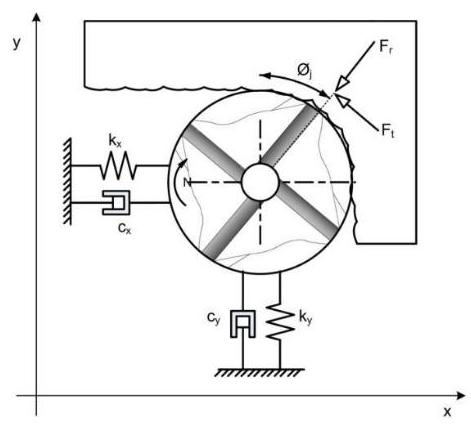
\includegraphics[max width=0.4\textwidth]{images/01948e67-2b92-7dd1-b16f-a9746c8d80be_2_588_1517_471_427_0.jpg}
\end{center}
\hspace*{3em} 

Fig. 1. Two DOF flexible end milling cutter model.

[Type here] IOP Conf. Series: Materials Science and Engineering 247 (2017) 012014 doi:10.1088/1757-899X/247/1/012014

\section*{A. Equations of motion}

The flexible tool model is assumed to be a spring mass system with dampers with 2 degrees of freedom. For simplicity the work-piece is considered to be rigid. Fig. 1 shows the 2 DOF-model of flexible multi-teeth milling cutter with simultaneous engagement. Simultaneous engagement refers to engagement of more than one cutting edge of the milling cutter. The tool is assumed to have straight flutes for simplicity in modeling of cutting forces. The radial and tangential cutting forces \(\left( {{\mathrm{F}}_{\mathrm{r}},{\mathrm{F}}_{\mathrm{t}}}\right)\) acting on a tooth can be expressed using the cutting coefficients \(\left( {{\mathrm{K}}_{\mathrm{t}},\mathrm{{Kr}}}\right)\) and chip width (h). The material dependent cutting coefficients can be found from standard machining data handbooks [1].

In local coordinates the forces \(\left( {{\mathrm{F}}_{\mathrm{r}},{\mathrm{F}}_{\mathrm{t}}}\right)\) are

\[
{\left\{  \begin{array}{l} {F}_{t} \\  {F}_{r} \end{array}\right\}  }_{j} = {\left\lbrack  \begin{matrix} {K}_{t}h\left( \theta \right) a \\  {K}_{t}{k}_{r}h\left( \theta \right) a \end{matrix}\right\rbrack  }_{j} = {\left\lbrack  \begin{matrix} {K}_{t}h\left( \theta \right) a \\  {F}_{t}{k}_{r} \end{matrix}\right\rbrack  }_{j} \tag{1}
\]

where \(\theta\) is the instantaneous angle made by the rotating end mill tooth (z-axis) referenced with respect to y axis and 'a' is the axial depth of cut (ADOC).

Transformation of Eqn. 1 to global coordinates results in resolution of forces on X and Y direction as shown below:

\[
{\left\{  \begin{array}{l} {\mathrm{F}}_{\mathrm{x}} \\  {\mathrm{F}}_{\mathrm{y}} \end{array}\right\}  }_{\mathrm{j}} = {\left\lbrack  \begin{matrix}  - \sin \left( \theta \right) &  - \cos \left( \theta \right) \\   - \cos \left( \theta \right) & \sin \left( \theta \right)  \end{matrix}\right\rbrack  }_{\mathrm{j}}{\left\{  \begin{array}{l} {\mathrm{F}}_{\mathrm{r}} \\  {\mathrm{F}}_{\mathrm{t}} \end{array}\right\}  }_{\mathrm{j}} \tag{2}
\]

The cutting tool dynamics of the end mill cutter is influenced by the parameters namely mass, stiffness and damping factor. The periodical vibrating force is induced by the regenerative effect of the tool. The equations of motion of the flexible tool system consisting of \(\mathrm{Z}\) cutting edges can be written as

\[
\ddot{\mathrm{x}} + 2{\zeta }_{\mathrm{x}}{\omega }_{\mathrm{{nx}}}\dot{\mathrm{x}} + {\omega }_{\mathrm{{nx}}}^{2}\mathrm{x} = \frac{1}{{\mathrm{\;m}}_{\mathrm{x}}}\mathop{\sum }\limits_{{\mathrm{j} = 0}}^{{\mathrm{Z} - 1}}{\mathrm{\;F}}_{\mathrm{{xj}}} = \frac{1}{{\mathrm{\;m}}_{\mathrm{x}}}{\mathrm{F}}_{\mathrm{x}}\left( \mathrm{t}\right)  \tag{3}
\]

\[
\ddot{\mathrm{y}} + 2{\zeta }_{\mathrm{y}}{\omega }_{\mathrm{{ny}}}\dot{\mathrm{y}} + {\omega }_{\mathrm{{ny}}}^{2}\mathrm{y} = \frac{1}{{\mathrm{\;m}}_{\mathrm{y}}}\mathop{\sum }\limits_{{\mathrm{j} = 0}}^{{\mathrm{Z} - 1}}{\mathrm{\;F}}_{\mathrm{{xj}}} = \frac{1}{{\mathrm{\;m}}_{\mathrm{y}}}{\mathrm{F}}_{\mathrm{y}}\left( \mathrm{t}\right)  \tag{4}
\]

where is \(\mathrm{m}\) the modal mass, \(\xi\) is the damping ratio and \({\omega }_{\mathrm{n}}\) is the natural angular frequency and \(\mathrm{F}\) is the cutting force. Depending on the immersion angle of the cut, a \(Z\) toothed cutter may engage with multiple teeth on the work piece. Hence the forces on every tooth computed are summed up to consider the effect of all the teeth engaged in the cut as shown in Eqns. 3 \& 4.

\section*{B. Computation of Chip thickness}

Evaluation of instantaneous forces requires computation of chip thickness. The instantaneous chip thickness \(\mathrm{h}\left( \theta \right)\) due to regenerative effect is calculated as follows.

In case of a smooth surface the chip thickness can be expressed as

\[
{\mathrm{h}}_{\mathrm{s}} = \mathrm{c}\sin \left( \theta \right)  \tag{5}
\]

where \(\mathrm{c}\) is the chip load or feed per tooth. Since the chip thickness changes due to the feedback effect of the previous pass (t-T), it is expressed in local coordinates u-v (u: radial direction) as

\[
{\mathrm{h}}_{\mathrm{d}} = {\mathrm{h}}_{\mathrm{s}} + \mathrm{u}\left( {\mathrm{t} - \mathrm{T}}\right)  - \mathrm{u}\left( \mathrm{t}\right)  \tag{6}
\]

where \(\mathrm{T}\) is the tooth passing period given by [Type here] IOP Conf. Series: Materials Science and Engineering 247 (2017) 012014 doi:10.1088/1757-899X/247/1/012014

\[
\mathrm{T} = \frac{60}{\mathrm{{NZ}}} \tag{7}
\]

with \(\mathrm{N}\) as the cutter speed in minutes. Though it is possible to use the \({\mathrm{h}}_{\mathrm{d}}\) directly to compute forces, for convenience it is expressed in the x-y global coordinate system using the transformation matrix.

\[
\mathrm{u}\left( \mathrm{t}\right)  =  - \mathrm{x}\left( \mathrm{t}\right) \sin \theta  - \mathrm{y}\left( \mathrm{t}\right) \cos \theta  \tag{8}
\]

\[
\mathrm{u}\left( {\mathrm{t} - \mathrm{T}}\right)  =  - \mathrm{x}\left( {\mathrm{t} - \mathrm{T}}\right) \sin \theta  - \mathrm{y}\left( {\mathrm{t} - \mathrm{T}}\right) \cos \theta  \tag{9}
\]

Substituting in the Eqn. 6 for \({\mathrm{h}}_{\mathrm{d}}\)

\[
{\mathrm{h}}_{\mathrm{d}} = \left( {{\mathrm{h}}_{\mathrm{s}} + \left\lbrack  {\mathrm{x}\left( \mathrm{t}\right)  - \mathrm{x}\left( {\mathrm{t} - \mathrm{T}}\right) }\right\rbrack  \sin \left( {\theta }_{\mathrm{i}}\right) }\right.  \tag{10}
\]

\[
\left. {+\left\lbrack  {\mathrm{y}\left( \mathrm{t}\right)  - \mathrm{y}\left( {\mathrm{t} - \mathrm{T}}\right) }\right\rbrack  \cos \left( {\theta }_{\mathrm{i}}\right) }\right)
\]

The above equation shows that the chip thickness is dependent of previous passes which makes the equation into a Delay Differential Equation (DDE).

\section*{C. Effect of intermittent cutting}

In machining with end-mills, the tool edge does not engage with work all the times. The tool engagement time is dependent on the angle of entry and exit. This produces intermittent cutting operation. To consider the effect of intermittent cutting action of the tooth of the milling cutter a unit step function \(\mathrm{g}\left( {\theta }_{\mathrm{i}}\right)\) is multiplied with the above equation. It must be noted that at any given point of time, depending on the number of tool edges and entry and exit angle, more than one cutting edge may be involved in the cutting operation.

\[
\mathrm{g}\left( \theta \right)  = \left\{  \begin{matrix} 1 & {\theta }_{\text{ entry }} < \theta  < {\theta }_{\text{ exit }} \\  0 & \text{ otherwise } \end{matrix}\right.  \tag{11}
\]

The angular position at any given instant \(t\) can be found by using the relation

\[
\theta \left( \mathrm{t}\right)  = \frac{{2\pi }\mathrm{{Nt}}}{60} + \frac{\mathrm{Z}{2\pi }}{\mathrm{N}} \tag{12}
\]

Use Eqn. 12 the instantaneous position of the tool edge can be computed. If it lies between the entry and exit angle of the work, forces can be obtained according to Eqn. 2 otherwise forces experienced from that edge will be zero according to Eqn. 11. Substituting the \({\mathrm{h}}_{\mathrm{d}}\) in the Eqn. 1 forces \({\mathrm{F}}_{\mathrm{x}}\) and \({\mathrm{F}}_{\mathrm{y}}\) can be computed from eqn.2. Subsequently eqns. 3 \& 4 can be solved numerically using R-K method.

\section*{III. STATE SPACE FORM OF DDE}

To solve a higher order differential equation, it must first be expressed as first order simultaneous differential equations. A state space form which is easy to implement in MATLAB software is used here. For the chatter equations (Eqns. 3 \& 4) the state variables can be expressed as follows

\[
{\mathrm{x}}_{1} = \mathrm{x} \tag{13}
\]

\[
{\mathrm{x}}_{2} = {\dot{\mathrm{x}}}_{1} \tag{14}
\]

and the simultaneous differential equations can be written as

\[
{\dot{\mathrm{x}}}_{1} = {\mathrm{x}}_{2}\text{ and } \tag{15}
\]

\[
{\dot{\mathrm{x}}}_{2} = \frac{1}{\mathrm{\;m}}\left( {\mathrm{\;F} - {\mathrm{{cx}}}_{2} - {\mathrm{{kx}}}_{1}}\right)  \tag{16}
\]

[Type here] IOP Conf. Series: Materials Science and Engineering 247 (2017) 012014 doi:10.1088/1757-899X/247/1/012014

\section*{IV. DELAY DIFFERENTIAL EQUATIONS}

Delay differential arise in all types of disciplines and it has received wide attention which has lead to the development of efficient solvers. Though DDEs are similar to ODEs, their solution procedure is different as the solution is dependent on its previous delay period(s). The delay period in chatter problems is a positive real number and multiple delay periods are common in chatter DDEs. Once the solution for the current delay period is computed, the sequence is continued for the next delay period. The solution at the previous time period is called as history in DDE terminology. While solving DDEs, discontinuous derivates may arise and require special treatment. Since the effect of low order discontinuities is more, it is tracked till it is smoothened out. Solvers usually calculate the discontinuities in advance and truncate the higher order discontinuities [15].

Runge-Kutta method is the most widely method used to solve DDEs however when used with constant step size it leads to poor error control. Modern solvers use variable step size, though choosing a proper step size without increasing computation burden is an important issue. Moreover it must be chosen to get an accurate approximation. Since DDE with variable step size require solution at previous times other than mesh points, interpolation of results is required. Cubic hermite interpolants are widely used in DDE solvers to obtain the solution everywhere in the interval. In this paper the solution for DDE is obtained using DDE23 which is proposed by Shampine [14]. The solver uses BS (23) pair with continuous extensions of R-K formulas which enables to compute solution at any given time ’t’. DDE23 also provides an powerful event capability which is useful to solve milling chatter problems with multiple cutting edges simultaneously acting together. However DDE23 is not suitable for variable time delays problems that occur due to varying speed and varying pitch.

\section*{V. SOLUTION PROCEDURE}

\section*{A.DDE interface}

In this section the implementation of chatter equations for DDE23 solver is explained using its standard interface. The dde23 function call is as follows

sol=dde23('ChtrddeFunc', [time delay], 'ChtrHistory', [tintial, tfinal], options, state); (17) where

1) ChtrddeFunc : a handle to function that defines the state space form of a delay differential equation (Eqns. 19 and 20).

2) [Time delay]: time delay which is equal to T according to Eqn. 7.

3) ChtrHistory: a handle to function for solution history

4) [Tintial tfinal]: the time span of integration which is user defined. Generally 0-3 seconds

5) Options: used for reentry

6) State: variable passed to trigger the start of a new integration.

The dde23 solver returns the solution 'sol' which is a structure consisting of time, solution 'y' and its derivative. The dde23 solver updates time ’t’ automatically and the adaptive increment to parameter ’t’ is chosen by the dde23.

\section*{B. Modeling chatter as function}

The first step to solve chatter equations consists of implementing the equations mentioned in section 2 as a function 'chtrddefunction'. The function comprises the chatter equations (Eqns. 17-20) expressed in state space form. To compute the forces at a given instant,’ \(t\) ’ the angular position of the tooth \(\left( \theta \right)\) has to be first found. Employing Eqn. 12 and looping through 1 to Z number of teeth, the instantaneous positions of the all the teeth can be calculated. Though the initial position can be at any random angle, for simplicity the initial position is assumed to coincide with positive \(\mathrm{Y}\) axis. When the location angle ’ \(\theta\) ’ lies between the ’ \({\theta }_{\text{ entry }}\) ’ and ’ \({\theta }_{\text{ exit }}\) ’ forces \({\mathrm{F}}_{\mathrm{x}},{\mathrm{F}}_{\mathrm{y}}\) are computed otherwise they are set to zero according to Eqn. 11. This sub- procedure is made as a loop and all the forces are summed according to the Eqns.3 \& 4.

\section*{[Type here]}

IOP Conf. Series: Materials Science and Engineering 247 (2017) 012014 doi:10.1088/1757-899X/247/1/012014

The chip thickness is computed according to Eqn.10. The history of previous values at (t-T) is provided by the \(\mathrm{Z}\) lag values which are passed to this function as an input parameter according to the syntax.

Table .1: Data for MATLAB simulation

\begin{center}
\adjustbox{max width=\textwidth}{
\begin{tabular}{|c|c|}
\hline
Natural freq. \({\omega }_{\mathrm{{nx}}},{\omega }_{\mathrm{{ny}}}\) (Hz) & 600, 660 \\
\cline{1-2}
Damping ratio \({\xi }_{\mathrm{x}}\) , \({\xi }_{\mathrm{y}}\) & 0.035, 0.035 \\
\cline{1-2}
Stiffness \({\mathrm{k}}_{\mathrm{x}}{\mathrm{k}}_{\mathrm{v}}\left( {\mathrm{N}/\mathrm{m}}\right)\) & 5600*10 \({}^{3}\) \\
\cline{1-2}
Number of teeth & 4 \\
\cline{1-2}
\({\mathrm{K}}_{\mathrm{t}}\left( \mathrm{{MPa}}\right) ,{\mathrm{K}}_{\mathrm{r}}\) & 600, 0.07 \\
\cline{1-2}
Milling type & Half immersion \\
\cline{1-2}
\hline
\end{tabular}
}
\end{center}

\section*{C. Defining history of chatter}

The second step is to define the history function. In most of the chatter problems the initial displacement profile is assumed to be ' 0 '. With this approach, it is possible to express the initial profile and its derivates using the history function.

\[
\mathrm{v} = \text{ ChtrHistory ( }\mathrm{t}\text{ , state) } \tag{18}
\]

where ’ \(v\) ’ is the vector of state variables computed for time ’ \(t\) ’. The history definition is used only during the first iteration and for subsequent integration histories; the values from DDE solution (Z lag values) are used.

\section*{D. Restarting integration after each tooth pass}

The next step is concerned with restarting of the integration. The integration of DDE cannot be continued indefinitely after every tooth passing period since the newly engaged tooth will encounter the profile left by the previous tooth. Hence the solution for the current and newly engaged tooth must consider the displacement profile left by the previous tooth and its derivative. This can be modeled using the event options of DDE23 through the ddeset command.

\[
\text{ options = ddeset('Event','ChtrEvents'); } \tag{19}
\]

where 'ChtrEvents' is a handle to the function which is similar to 'Chtrddefunction' function. The function compares the state value with the instantaneous time 't' and when they become equal, an event is triggered to stop the current integration.

To obtain a meaningful result, the numerical integration process must be executed for a certain time span set by the user. During this time, the dde23 solver is called repetitively in a while loop at time intervals equal to the tooth passing period. In each iteration, the parameter 'state' is incremented in integer increments of time delay period. Thus the events function triggers the integration to stop when the state values equals the tooth passing period and the solution is placed in sol variable. Comparing the time 't' from the solution structure with the given max time span the execution of while loop can be controlled. For all the subsequent calls made by dde23 solver, the solution returned by the previous call is passed as history. The starting value of the time span is updated with the final time value available at the end of solution structure. The summary is shown in figure 2.

[Type here] IOP Conf. Series: Materials Science and Engineering 247 (2017) 012014 doi:10.1088/1757-899X/247/1/012014

\begin{center}
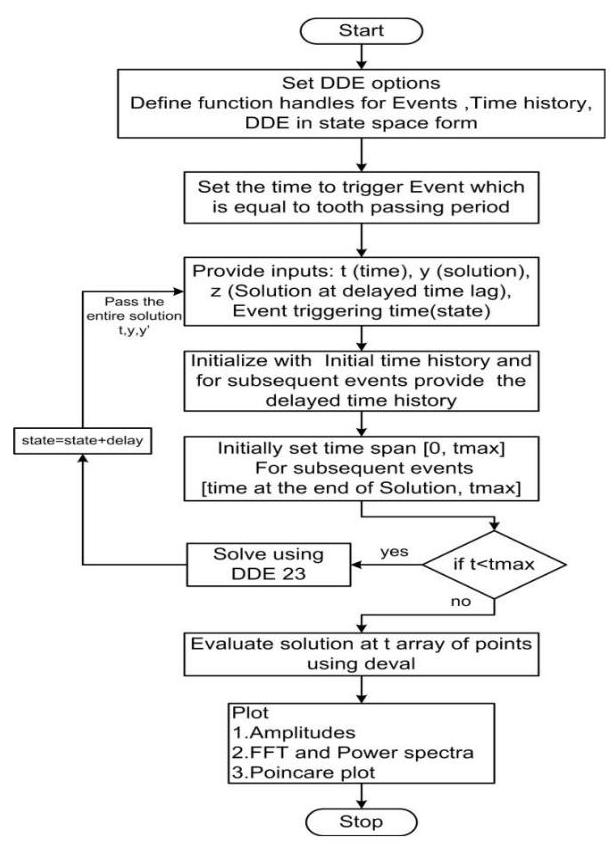
\includegraphics[max width=0.5\textwidth]{images/01948e67-2b92-7dd1-b16f-a9746c8d80be_7_518_284_614_844_0.jpg}
\end{center}
\hspace*{3em} 

Fig. 2. Summary of the procedure

\section*{VI .RESULTS AND DISCUSSION}

Table 1 shows the data used to evaluate the proposed procedure. A straight fluted end milling cutter is used for simplicity. Fig. 3 shows the trimmed stability lobe diagram computed using the conventional approach with these parameters [16, 17]. The diagram can be divided into two regions namely 1) stable region with no chatter and 2) unstable regions with chatter. It must be noted that non-linearity effects are ignored in this approach to arrive closed \(\mathrm{m}\) solution of onset of chatter. Using procedures mentioned in the previous section, the chatter delay differential equations are solved and the time domain solutions are computed for various speeds and depth of cut. Figs. 4 \& 5 show the displacement profile along X and Y direction computed for a speed of 3000 rpm with depth of cut \(1\mathrm{\;{mm}}\) . From these figures one can find that the diverging profile leads to instability resulting in chatter.

\begin{center}
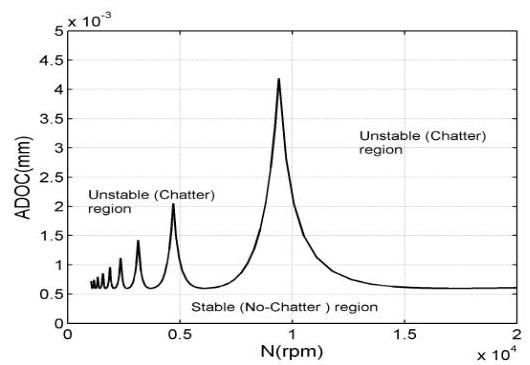
\includegraphics[max width=0.4\textwidth]{images/01948e67-2b92-7dd1-b16f-a9746c8d80be_7_546_1546_530_365_0.jpg}
\end{center}
\hspace*{3em} 

Fig. 3. Stability lobe diagram using Table 1

[Type here] IOP Conf. Series: Materials Science and Engineering 247 (2017) 012014 doi:10.1088/1757-899X/247/1/012014

\begin{center}
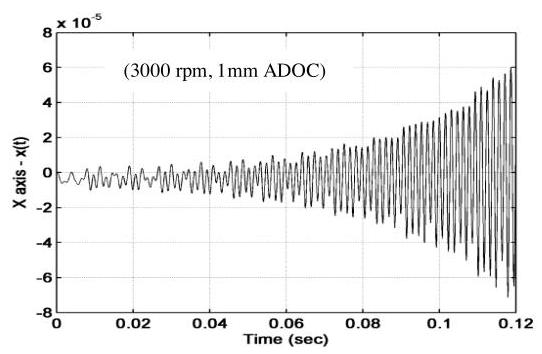
\includegraphics[max width=0.4\textwidth]{images/01948e67-2b92-7dd1-b16f-a9746c8d80be_8_551_285_542_354_0.jpg}
\end{center}
\hspace*{3em} 

Fig. 4. X-Displacement profile

\begin{center}
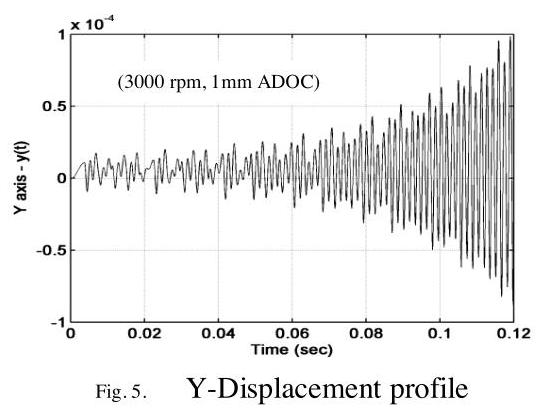
\includegraphics[max width=0.4\textwidth]{images/01948e67-2b92-7dd1-b16f-a9746c8d80be_8_545_731_542_411_0.jpg}
\end{center}
\hspace*{3em} 

However for the speed of 10000 rpm with \(3\mathrm{\;{mm}}\) depth of cut, the \(\mathrm{X}\) displacement profile clearly shows diverging characteristics though the amplitude is very small (Fig. 6). The Y-axis profile shows a near stable profile though its diverging trends are not visible (Fig. 7). However, according to conventional stability lobe diagram (Fig. 3), this data point lies in the stable region. This shows the difference between the time domain approach and stability lobe approach since the later does not model the non-linearities. A stable cut at 15000 rpm and 0.5 mm depth of cut is observed (Figure 8). The computation time for all the above cases is observed to average between 30 seconds and 40 seconds with a Pentium Celeron processor with 2GB RAM. Due to variable step size in solving the chatter delay differential equation, the time taken to obtain time domain solution varies from case to case. This method is preferred for constant delays problems which is a common in high speed machining.

\begin{center}
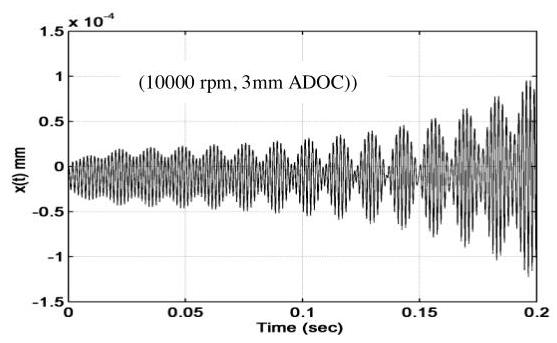
\includegraphics[max width=0.4\textwidth]{images/01948e67-2b92-7dd1-b16f-a9746c8d80be_8_535_1593_557_343_0.jpg}
\end{center}
\hspace*{3em} 

Fig. 6. Displacement profile (10000 rpm, 3mm ADOC)

\(\left( {{10000}\mathrm{{rpm}},3\mathrm{{mm}}\mathrm{{ADOC}}}\right) )\)

[Type here] IOP Conf. Series: Materials Science and Engineering 247 (2017) 012014 doi:10.1088/1757-899X/247/1/012014

\begin{center}
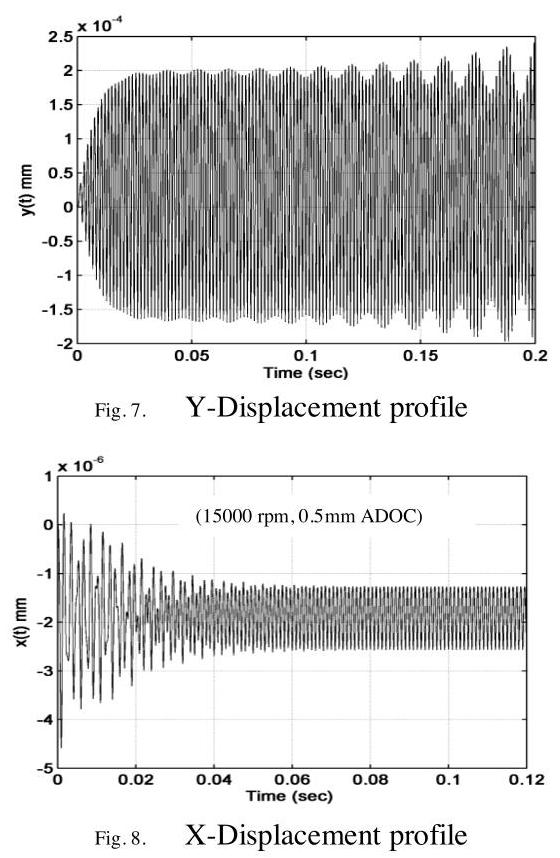
\includegraphics[max width=0.4\textwidth]{images/01948e67-2b92-7dd1-b16f-a9746c8d80be_9_546_263_560_858_0.jpg}
\end{center}
\hspace*{3em} 

Further, it is possible to analyze the chatter conditions according to frequency spectrum computed from the displacement profile. From the Fig. 10 it can be noticed that the multiple frequency peaks leads to chatter condition. A clear peak frequency corresponding to the tool path frequency indicates chatter free machining process. With simple modification the proposed method can be extended to analyze chatter in turning process.

The procedures developed in this article will be helpful for the study of non-linear chatter problems in high speed machining. The tool displacement profiles along \(\mathrm{x}\) and \(\mathrm{y}\) provide inputs for constructing bifurcation diagram and the relevance of onset of chatter can be analyzed based on floquet theory. Useful inferences can be made by comparing the results with conventional stability lobe diagram. In addition the time history of the previous periods provide useful information for analysis.

\begin{center}
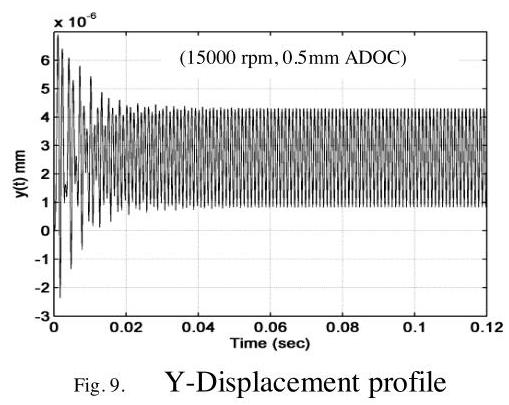
\includegraphics[max width=0.4\textwidth]{images/01948e67-2b92-7dd1-b16f-a9746c8d80be_9_567_1492_509_405_0.jpg}
\end{center}
\hspace*{3em} 

[Type here] IOP Conf. Series: Materials Science and Engineering 247 (2017) 012014 doi:10.1088/1757-899X/247/1/012014

\begin{center}
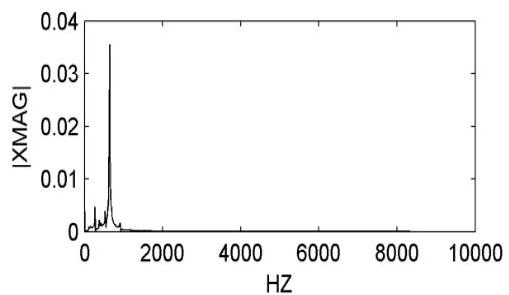
\includegraphics[max width=0.4\textwidth]{images/01948e67-2b92-7dd1-b16f-a9746c8d80be_10_567_255_509_295_0.jpg}
\end{center}
\hspace*{3em} 

(a) Chatter FFT profile showing multiple frequencies (3000 rpm, 1 mm ADOC)

\begin{center}
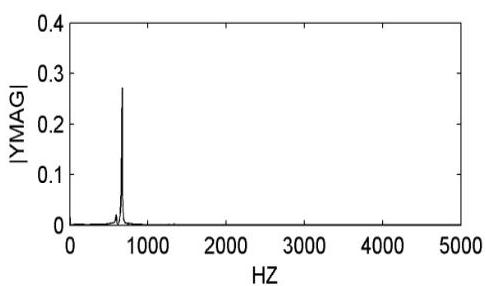
\includegraphics[max width=0.4\textwidth]{images/01948e67-2b92-7dd1-b16f-a9746c8d80be_10_587_657_486_286_0.jpg}
\end{center}
\hspace*{3em} 

(c) No chatter FFT profile showing one dominant frequency (10000 rpm, 3mm ADOC)

Fig. 10. Analysis of chatter from FFT profiles from time domain results

\section*{VII. CONCLUSIONS}

1. A new approach to obtain time domain solution to chatter problems with non-linearities is proposed in this paper. A time domain solution for an example problem is illustrated.

2. The solver used in this method equips with adaptive time step size and error control methods resulting in a more accurate solution. It is suitable for multiple time delays and problems with added DOFs. It is possible to construct Poincare plot as derivatives are available in the solution structure.

3. Though a straight flute cutter is used for analysis, the proposed method can be extended to helical flute cutter by modifying the program segment that computes forces.

4. The proposed method is suitable to solve problem with an initial profile.

5. The proposed method can be used as an alternate to conventional stability lobe diagram with loops.

\section*{REFERENCES}

[1] H. Schulz and T. Moriwaki, "High-speed Machining", Annals of the ClRP, Vol. 41, pp.637- 643,1992

[2] M. Sekar, V.N. Narayanan and Seung-Han Yang, "Design of jerk bounded feedrate with ripple effect for adaptive NURBS interpolator", International Journal of Advanced Manufacturing Technology, Vol.37, No. 5 pp. 545-552, 2008.

[3] J. Tlusty, "Manufacturing Process and Equipment," Prentice Hall, USA, 2000.

[4] H.E. Meritt, "Theory of Self-Excited Machine Tool Chatter," ASME J. Engg. Industry, 87, pp. 447- 454, 1965.

[5] S.A. Tobias, "Machine tool Vibration," Blackie, London, 1965

[6] R. Sridhar, R.E. Hohn, and W. Long, "A General Formulation of the Milling Process Equation," ASME J. Engg Industry, 90, pp. 317-324, 1968.

[Type here] IOP Conf. Series: Materials Science and Engineering 247 (2017) 012014 doi:10.1088/1757-899X/247/1/012014

[7] I. Minis and R. Yanushevsky, "A new theoretical approach for the prediction of machine tool chatter in milling," ASME J.Engg Industry, 115, pp. 1-8, 1993.

[8] Y. Altintas and E. Budak, "Analytical prediction of stability lobes in milling," Annals of CIRP, Vol. 44, pp. 357-362, 1995.

[9] M.X. Zhao and B. Balachandran, "Dynamics and stability of milling process," Int. J of solids and structures, Vol. 38, pp. 2233-2248, 2001.

[10] H. Li., and X. Li, "Modeling of simulation of chatter in milling using a predictive force model," Int J. Mach Tools and Manuf., Vol. 40, pp. 2047-2071, 2000.

[11] T. Insperger, J. Gradisek, M. Kalveram, G. Stepan, K. Winert and E. Govekar, "Machine Tool Chatter and Surface Location Error in Milling Processes," ASME Journal of Mfg Science, Vol.128, pp. 913-920, 2006.

[12] W. Andrzej, R. Rafal and W. Jerzy, "The concept of active elimination of vibrations in milling process", Procedia CIRP, Vol. 31, pp. 82 – 87, 2015.

[13] J. H. E. Cartwright and O. Prio, "Dynamics of Runge-Kutta methods," Int. Journal of Bifurcation and Chaos, Vol. 2, pp. 427-449, 2002

[14] W. H. Enright, D.J. Higham, B. Owren and P.W. Sharp, "A survey of Explicit R-K method," TR 291/94, Depart. of Comp. Sci., University of Toronto, 1994.

[15] C.T.H. Baker, C.A.H. Paul and D.R. Willé, "Issues in the Numerical Solution of Evolutionary Delay Differential Equations," Adv. Comput. Math., 3, pp. 171–196,1995.

[16] L.F. Shampine and S. Thomson“Solving DDEs in MATLAB,” Applied Numerical Mathematics, 37, pp. 441-458, 2001.

[17] L.F. Shampine, I. Gladwell, S. Thomson, "Solving ODES with MATLAB," Cambridge University press, UK, 2003.

[18] M. Sekar, J. Srinivas, N. Kang and S.H. Yang, "An Integrated Approach to the Improvement of Stability Lobes," Int.. J. of Precision Engineering and Manufacturing, Vol. 9, pp: 83-85, 2008.

[19] M. Sekar, J. Srinivas, K.R. Rama Kotaiah and Seung-Han Yang, "Stability Analysis of Turning Process with Tailstock-Supported Workpiece," Int. J. of Advanced manufacturing Technology, Vol. 43, pp. 862-871, 2009.
\end{document}